\documentclass[tikz,border=10pt]{standalone}
\begin{document}
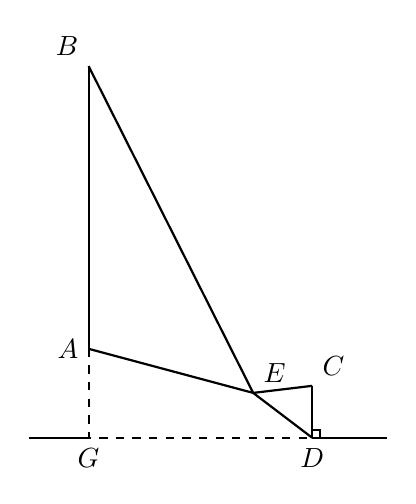
\begin{tikzpicture}[line width=0.8pt]
  \coordinate (B) at (1.04,4.72);
  \coordinate (A) at (1.04,1.13);
  \coordinate (G) at (1.04,0);
  \coordinate (D) at (3.88,0);
  \coordinate (C) at (3.88,0.66);
  \coordinate (E) at (3.13,0.57);
  \coordinate (L1) at (0.28,0);
  \coordinate (L2) at (4.83,0);

  \draw (L1) -- (G);
  \draw (D) -- (L2);
  \draw[dashed] (A) -- (G) -- (D);
  \draw (B) -- (A);
  \draw (B) -- (E);
  \draw (A) -- (E);
  \draw (E) -- (C);
  \draw (C) -- (D);
  \draw (E) -- (D);
  \draw (3.88,0) -- (3.98,0) -- (3.98,0.1) -- (3.88,0.1);

  \node[above left] at (B) {$B$};
  \node[left] at (A) {$A$};
  \node[below] at (G) {$G$};
  \node[below] at (D) {$D$};
  \node[above right] at (C) {$C$};
  \node[above right] at (E) {$E$};
\end{tikzpicture}
\end{document}
